% Shared standalone design for the editable figure reconstructions.
\documentclass[tikz,border=5pt,10pt]{standalone}
\usepackage[T1]{fontenc}
\usepackage[utf8]{inputenc}
\usepackage{newpxtext,newpxmath}
\usepackage[scaled=.94]{sourcesanspro}
\usepackage{pgfplots}
\pgfplotsset{compat=1.18}
\usetikzlibrary{arrows.meta,calc,positioning,decorations.pathreplacing,
  decorations.markings,patterns,matrix,shapes.geometric,fit,backgrounds,
  intersections,angles,quotes}
\definecolor{ink}{HTML}{203746}
\definecolor{accent}{HTML}{146C78}
\definecolor{muted}{HTML}{667780}
\definecolor{signalred}{HTML}{B94B44}
\color{ink}
\tikzset{>=Latex,line width=.8pt,
  every node/.style={font=\small},
  axis/.style={->,draw=muted,line width=.5pt},
  guide/.style={draw=muted,dashed,line width=.45pt},
  curve/.style={draw=accent,line width=1pt},
  marker/.style={circle,fill=accent,inner sep=1.5pt},
  labelbox/.style={fill=white,inner sep=2pt}}

\begin{document}
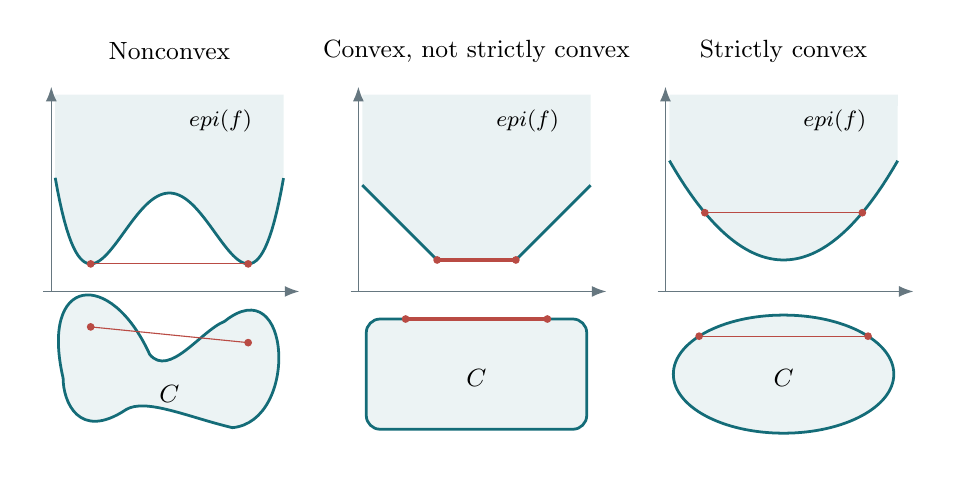
\begin{tikzpicture}

\path[use as bounding box] (-1.8,-2.2) rectangle (9.7,3.35);
\begin{scope}[shift={(0.0,0)}]
\node at (0,3.05) {Nonconvex};
\fill[accent!9] (-1.45,2.5) -- plot[domain=-1.45:1.45,samples=101] (\x,{.9*(\x*\x-1)^2+.35}) -- (1.45,2.5) -- cycle;
\draw[axis] (-1.6,0) -- (1.65,0); \draw[axis] (-1.5,0) -- (-1.5,2.6);
\draw[curve] plot[domain=-1.45:1.45,samples=101] (\x,{.9*(\x*\x-1)^2+.35});
\node[font=\footnotesize] at (.65,2.16) {$\operatorname{epi}(f)$};
\draw[signalred] (-1,.35)--(1,.35);\fill[signalred] (-1,.35) circle (1.4pt) (1,.35) circle (1.4pt);
\draw[curve,fill=accent!8] (-1.35,-1.1) .. controls (-1.65,.2) and (-.75,.3) .. (-.25,-.8) .. controls (0,-1.1) and (.4,-.5) .. (.7,-.38) .. controls (1.55,.3) and (1.65,-1.65) .. (.8,-1.73) .. controls (.25,-1.6) and (-.3,-1.35) .. (-.55,-1.5) .. controls (-1.15,-1.9) and (-1.35,-1.4) .. cycle;
\draw[signalred] (-1,-.45)--(1,-.65);\fill[signalred] (-1,-.45) circle (1.4pt) (1,-.65) circle (1.4pt);
\node at (0,-1.3) {$C$};
\end{scope}
\begin{scope}[shift={(3.9,0)}]
\node at (0,3.05) {Convex, not strictly convex};
\fill[accent!9] (-1.45,2.5) -- plot[domain=-1.45:1.45,samples=101] (\x,{max(abs(\x)-.5,0)+.4}) -- (1.45,2.5) -- cycle;
\draw[axis] (-1.6,0) -- (1.65,0); \draw[axis] (-1.5,0) -- (-1.5,2.6);
\draw[curve] plot[domain=-1.45:1.45,samples=101] (\x,{max(abs(\x)-.5,0)+.4});
\node[font=\footnotesize] at (.65,2.16) {$\operatorname{epi}(f)$};
\draw[signalred,line width=1.4pt] (-.5,.4)--(.5,.4);\fill[signalred] (-.5,.4) circle (1.4pt) (.5,.4) circle (1.4pt);
\draw[curve,fill=accent!8,rounded corners=5pt] (-1.4,-1.75) rectangle (1.4,-.35);
\draw[signalred,line width=1.4pt] (-.9,-.35)--(.9,-.35);\fill[signalred] (-.9,-.35) circle (1.4pt) (.9,-.35) circle (1.4pt);\node at (0,-1.1) {$C$};
\end{scope}
\begin{scope}[shift={(7.8,0)}]
\node at (0,3.05) {Strictly convex};
\fill[accent!9] (-1.45,2.5) -- plot[domain=-1.45:1.45,samples=101] (\x,{.6*\x*\x+.4}) -- (1.45,2.5) -- cycle;
\draw[axis] (-1.6,0) -- (1.65,0); \draw[axis] (-1.5,0) -- (-1.5,2.6);
\draw[curve] plot[domain=-1.45:1.45,samples=101] (\x,{.6*\x*\x+.4});
\node[font=\footnotesize] at (.65,2.16) {$\operatorname{epi}(f)$};
\draw[signalred] (-1,1)--(1,1);\fill[signalred] (-1,1) circle (1.4pt) (1,1) circle (1.4pt);
\draw[curve,fill=accent!8] (0,-1.05) ellipse (1.4 and .75);
\draw[signalred] ({1.4*cos(140)},{-1.05+.75*sin(140)})--({1.4*cos(40)},{-1.05+.75*sin(40)});
\fill[signalred] ({1.4*cos(140)},{-1.05+.75*sin(140)}) circle (1.4pt) ({1.4*cos(40)},{-1.05+.75*sin(40)}) circle (1.4pt);\node at (0,-1.1) {$C$};
\end{scope}

\end{tikzpicture}
\end{document}
